%%%%%%%%%%%%%%%%%%%%%%%%%%%%%%%%%%%%%%%%%
% baposter Portrait Poster
% LaTeX Template
% Version 1.0 (15/5/13)
%
% Created by:
% Brian Amberg (baposter@brian-amberg.de)
%
% This template has been downloaded from:
% http://www.LaTeXTemplates.com
%
% License:
% CC BY-NC-SA 3.0 (http://creativecommons.org/licenses/by-nc-sa/3.0/)
%
%%%%%%%%%%%%%%%%%%%%%%%%%%%%%%%%%%%%%%%%%

%----------------------------------------------------------------------------------------
%	PACKAGES AND OTHER DOCUMENT CONFIGURATIONS
%----------------------------------------------------------------------------------------

\documentclass[a0paper,portrait]{baposter}

\usepackage[font=small,labelfont=bf]{caption} % Required for specifying captions to tables and figures
\usepackage{booktabs} % Horizontal rules in tables
\usepackage{relsize} % Used for making text smaller in some places
\usepackage{graphicx}

\graphicspath{{figures/},{images/},{img/},{../HandmadeFigures/},{./}} % Directory in which figures are stored


\usepackage{tikz}
\usepackage{setspace}
\usepackage{multirow}
\usepackage{hyperref}

\usepackage{amsmath}
\usepackage{amsfonts}
\usepackage{amsthm}
\usepackage{bm}

\usepackage{enumitem}

\usepackage{gnuplot-lua-tikz}
\usepackage{tikz}
\usetikzlibrary{shapes,snakes,patterns}

% Define block styles
\tikzstyle{decision} = [diamond, draw, fill=blue!20, 
text width=6em, text badly centered, node distance=3cm, inner sep=0pt]
\tikzstyle{block} = [rectangle, draw, fill=blue!20, 
text width=15em, text centered, rounded corners, minimum height=4em]
\tikzstyle{block2} = [rectangle, draw, fill=blue!20, 
text width=25em, text centered, rounded corners, minimum height=4em]
\tikzstyle{block3} = [rectangle, draw, fill=blue!20, 
text width=20em, text centered, rounded corners, minimum height=4em]
\tikzstyle{block4} = [rectangle, draw, fill=blue!20, 
text width=7em, text centered, rounded corners, minimum height=4em]
\tikzstyle{block5} = [rectangle, draw, fill=blue!20, 
text width=15em, text centered, rounded corners, minimum height=4em]
\tikzstyle{block6} = [rectangle, draw, fill=blue!20, 
text width=25em, text centered, rounded corners, minimum height=4em]
\tikzstyle{line} = [draw, -latex']
\tikzstyle{cloud} = [draw, ellipse,fill=red!20, node distance=3cm,
minimum height=4em]


%=======================================================================================
% copied from presentation


% Corporate colors
\definecolor{tudCyan}{RGB}{61,152,222}
\definecolor{tudBlack}{RGB}{0,0,0}
\definecolor{tudWhite}{RGB}{255,255,255}
% Basic colors
\definecolor{tudSeaGreen}{RGB}{111,189,165}
\definecolor{tudGreen}{RGB}{39,131,142}
\definecolor{tudDarkBlue}{RGB}{34,70,122}
\definecolor{tudPurple}{RGB}{36,46,131}
\definecolor{tudTurquoise}{RGB}{50,154,179}
\definecolor{tudSkyBlue}{RGB}{130,187,206}
% Accent colors
\definecolor{tudLavender}{RGB}{121,150,180}
\definecolor{tudOrange}{RGB}{216,130,62}
\definecolor{tudWarmPurple}{RGB}{110,50,122}
\definecolor{tudFuchsia}{RGB}{178,72,146}
\definecolor{tudBrightGreen}{RGB}{183,200,34}
\definecolor{tudYellow}{RGB}{247,234,151}
%=======================================================================================


\definecolor{bordercol}{RGB}{40,40,40} % Border color of content boxes
\definecolor{headercol1}{RGB}{186,215,230} % Background color for the header in the content boxes (left side)
\definecolor{headercol2}{RGB}{80,80,80} % Background color for the header in the content boxes (right side)
\definecolor{headerfontcol}{RGB}{0,0,0} % Text color for the header text in the content boxes
%\definecolor{boxcolor}{RGB}{186,215,230} % Background color for the content in the content boxes
\definecolor{boxcolor}{RGB}{250,250,250}

\begin{document}
	
	
	\begin{poster}{
			grid=false,
			borderColor=tudBlack, % Border color of content boxes
			headerColorOne=headercol1, % Background color for the header in the content boxes (left side)
			headerColorTwo=tudCyan, % Background color for the header in the content boxes (right side)
			headerFontColor=headerfontcol, % Text color for the header text in the content boxes
			boxColorOne=boxcolor, % Background color for the content in the content boxes
			headershape=roundedright, % Specify the rounded corner in the content box headers
			headerfont=\Large\sf\bf, % Font modifiers for the text in the content box headers
			textborder=rectangle,
			background=none,
			headerborder=open, % Change to closed for a line under the content box headers
			boxshade=plain,
			headerheight=0.13\textheight
		}
		{}
		%
		%----------------------------------------------------------------------------------------
		%	TITLE AND AUTHOR NAME
		%----------------------------------------------------------------------------------------
		%
		{\sf\bf\smaller Semi implicit solver for high fidelity LES/DNS solutions of reacting flows} % Poster title
		{\vspace{0.5em} A.Surapaneni, D. Mira \\
			\vspace{1mm}{\footnotesize(anurag.surapaneni@bsc.es)\\} 
			\vspace{2mm}Barcelona Supercomputing Center} %\\ % Author names
		{
\includegraphics[scale=0.3]{Logos/BSC_logo_280.jpeg}} % University/lab logo
		
		
		%----------------------------------------------------------------------------------------
		%	ABSTRACT
		%----------------------------------------------------------------------------------------
		
		\headerbox{Abstract}{name=abstract,span=1,column=0,row=0}
		{
        
        \smaller
        
        A semi-implicit/point-implicit stiff solver (ODEPIM) for integrating chemistry in context of high fidelity LES/DNS simulations is presented. An overview of the algorithm and its numerical formulation is discussed. The solver is compared against state-of-the-art multi-order implicit solver (CVODE) in terms of accuracy and cost. It was found that for typical LES/DNS timestep sizes ODEPIM was about one order faster than CVODE, which makes it a compelling alternative. ODEPIM, as mentioned in the literature depends on a fixed sub-timestep to do the integration, a modification to determine the sub-timestep size is proposed making the solver dynamic and enabling greater speedup. A triple flame case is solved using the reference and modified ODEPIM solvers and is compared against the solution obtained from CVODE. Number of iterations of the dynamic ODEPIM method were found to correlate to the most reacting regions in the flame, however, even in these regions, dynamic ODEPIM was faster than the reference ODEPIM solver. 
 

        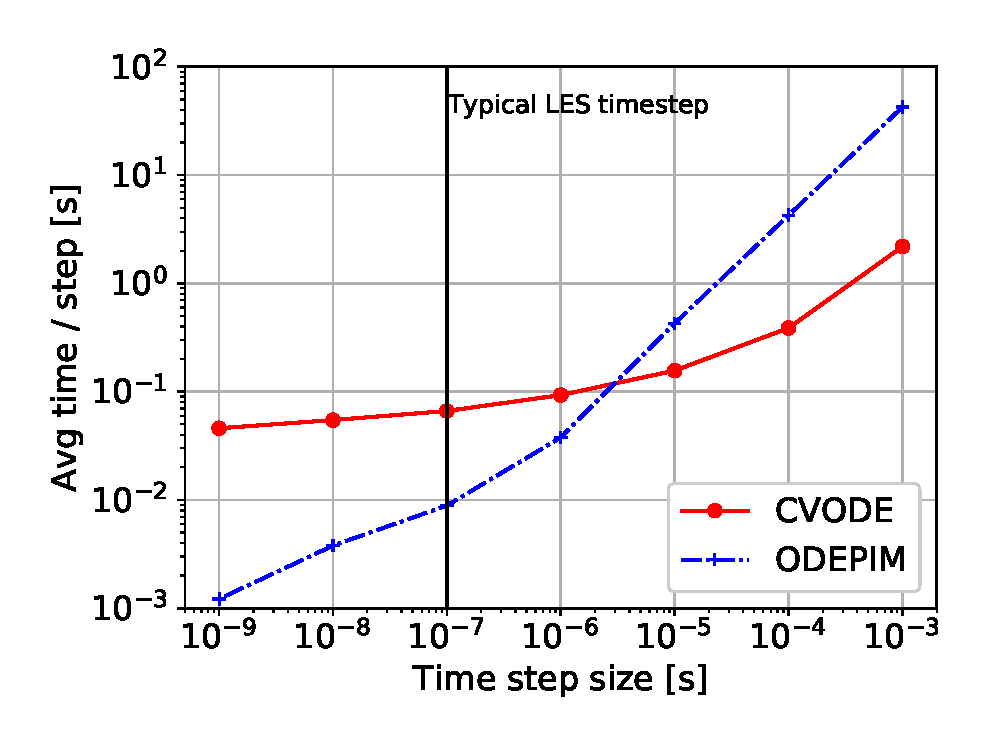
\includegraphics[width=0.8\linewidth]{time.eps}
        \caption{Cost per timestep size - CVODE v/s ODEPIM}

		}
		
		
		%----------------------------------------------------------------------------------------
		%	GOVERNING EQUATIONS
		%----------------------------------------------------------------------------------------
		
		\headerbox{Mathematical Model}{name=GovEq,span=1,column=0, below=abstract}{ % To reduce this block to 1 column width, remove 'span=2'
			
		
			\begin{equation}
                Y_{k}^{N+1,m} = \frac{Y_{k}^N + \omega^{+}_Y_{k}^{N,m} \Delta t}{1 + \frac{ \omega^{-}_ Y_{k}^{N,m} \Delta t}{Y_{k}^{N,m}}} 
                \label{eq:pro4}
            \end{equation}

            \begin{equation}
                \epsilon =  \underset{1\leq k \leq Niter}{max} \left(1 - \frac{log_{10}Y_{k}^{N,m}}{log_{10}Y_{k}^{N,m+1}}\right)  < \epsilon_{tol}     
                \label{eq:pro5}
            \end{equation}
            $Y_{k}$ - species mass fraction | $ \omega^{+/-}_Y_{k}$ - species source | $\Delta t$ - timestep size  | $\epsilon$ error to be minimised

				
		}
		

			\headerbox{Algorithm}{name=algo,span=1,column=0, below=GovEq}{ % To reduce this block to 1 column width, remove 'span=2'
		\resizebox{7cm}{10cm}{%
            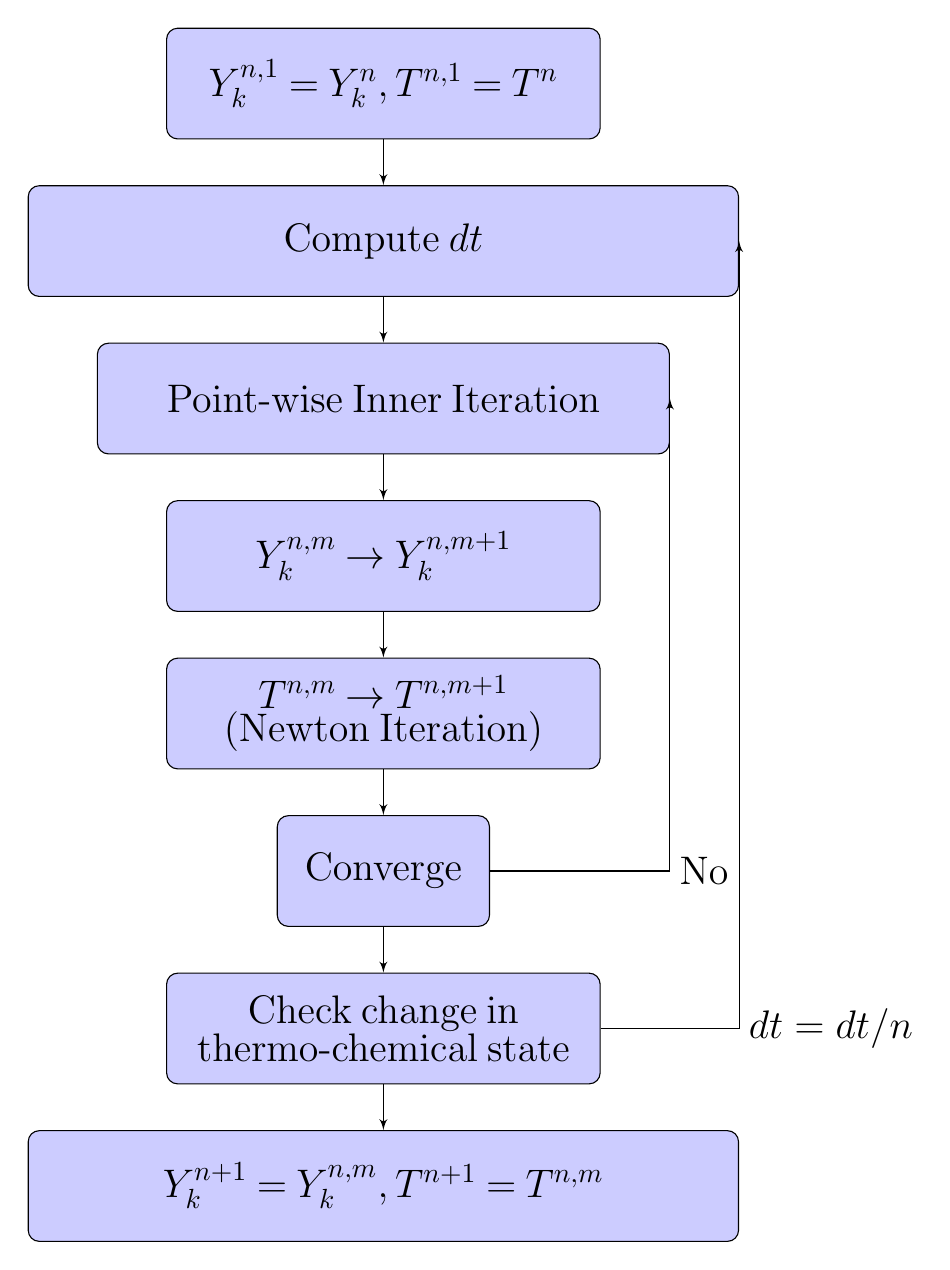
\begin{tikzpicture}[node distance = 2.0cm, auto,scale=0.30]
    % nodes
                \node [block] (initial) {\Large $Y_{k}^{n,1}$ = $Y_{k}^{n},T^{n,1} $ = $T^{n}$};
                \node [block6, below of = initial] (init) {\Large Compute $dt$};
                \node [block3, below of = init] (iter) {\Large Point-wise Inner Iteration};
                \node [block, below of = iter] (init2) {\Large $Y_{k}^{n,m}$ $\rightarrow$  $Y_{k}^{n,m+1}$};
                \node [block, below of = init2] (init3) {\Large $T^{n,m}$ $\rightarrow$ $T^{n,m+1}$ (Newton Iteration)};
                \node [block4, below of = init3] (conv) {\Large Converge};
                \node [block5, below of = conv] (conv2) {\Large Check change in thermo-chemical state};
                \node [block2, below of = conv2] (tdt) {\Large \Large $Y_{k}^{n+1}$ = $Y_{k}^{n,m},T^{n+1} $ = $T^{n,m}$};
    % edges
                \path [line] (initial) -- (init);
                \path [line] (init) -- (iter);
                \path [line] (iter) -- (init2);
                \path [line] (init2) -- (init3);
                \path [line] (init3) -- (conv);
                \path [line] (conv) -- (conv2);
                \path [line] (conv2) -- (tdt);
                \path [line] (conv2.east) -| node [anchor=west] {\Large $dt = dt/n $} (init.east);
                \path [line] (conv.east) -| node [anchor=west]               {\Large No}  (iter.east);
            \end{tikzpicture} 
				
		}	
	}
		
		%----------------------------------------------------------------------------------------
		%	COMPUTATIONAL SETUP
		%----------------------------------------------------------------------------------------
		
		
		
		
		
		
		
		
		
		%----------------------------------------------------------------------------------------
		%	REFERENCES
		%----------------------------------------------------------------------------------------

		

		%----------------------------------------------------------------------------------------
		%	FLAMELETS
		%----------------------------------------------------------------------------------------
		
		\headerbox{PSR - ODEPIM}{name=flamelet,span=2,column=1,row=0}{ % To reduce this block to 1 column width, remove 'span=2'
			\begin{minipage}{0.3\linewidth}
			    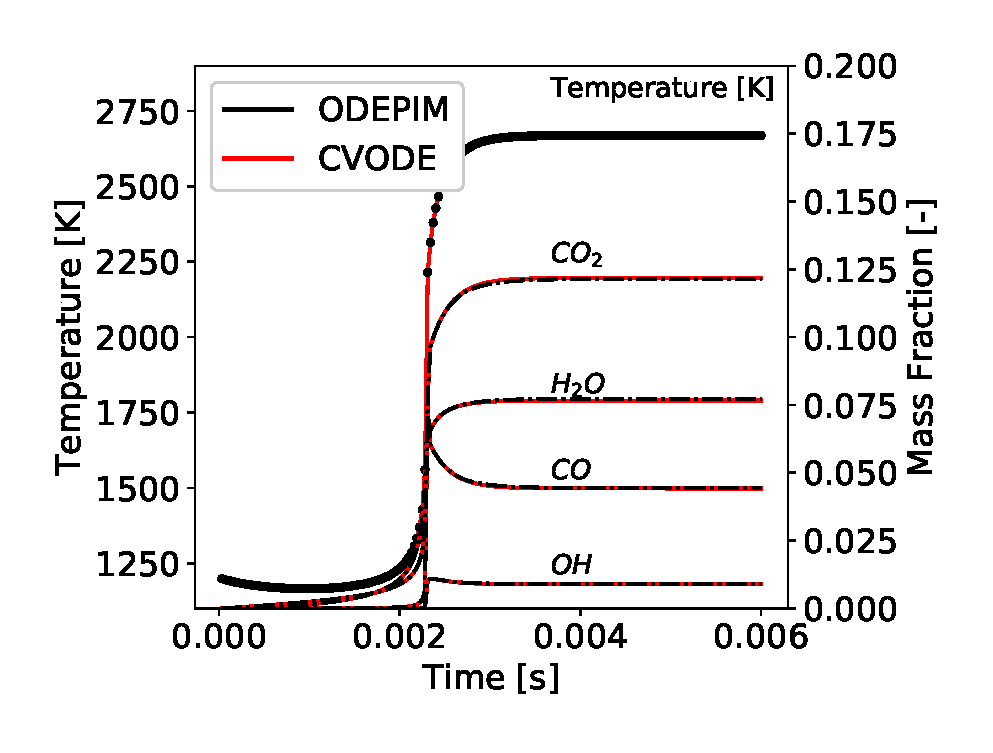
\includegraphics[width=\linewidth]{vali.eps}
			\end{minipage}
			\begin{minipage}{0.3\linewidth}
			   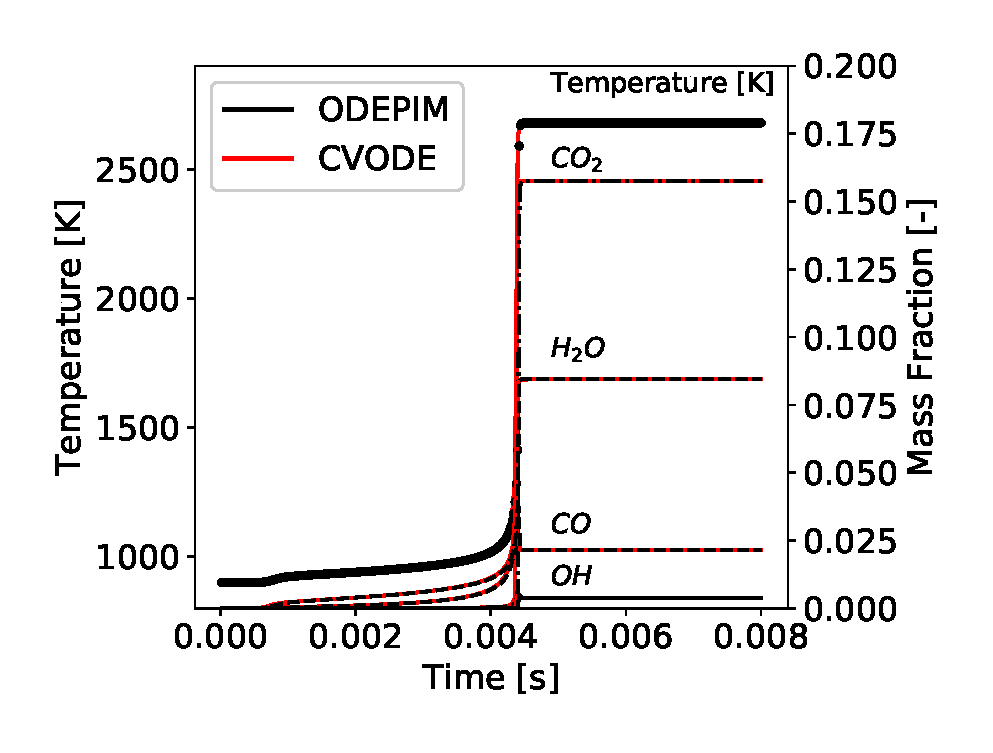
\includegraphics[width=\linewidth]{vali2.eps}
			\end{minipage}
			\begin{minipage}{0.4\linewidth}
			    \smaller
			    \begin{itemize}
		       	\setlength\itemsep{-0.3em}
		       	\item Case Parameters:
		       	\vspace{-0.7em}
		       	\begin{itemize}
		       	    \setlength\itemsep{-0.3em}
		       	    \item Stichiometeric N-Heptane/Air
		       	    \item Temperature - $1200$ [K], $900$ [k]
		       	    \item Pressure - 16 bar
		       	    \item Mechanism - Skeletal N-Heptane\\ \cite{lu2006linear} (188 species, 1719 reactions)
		       	\end{itemize}
		       	\item Low Mach solver with  \\
		       	      Strang Splitting \cite{vazquez2016alya}
		       	\item ODEPIM Tolerance = $1e-5$
		       	\item Key Variables - Dynamic ODEPIM \\ $Y_{OH}$, Temperature
		       \end{itemize}
			\end{minipage}
			
			
			
		}
		
		
		%----------------------------------------------------------------------------------------
		%	VALIDATION
		%----------------------------------------------------------------------------------------
		
		\headerbox{Odepim: Typical timestep }{name=validation,span=1,column=1,below=flamelet}{ % To reduce this block to 1 column width, remove 'span=2'
		

		    \begin{minipage}{1.0\linewidth}
			    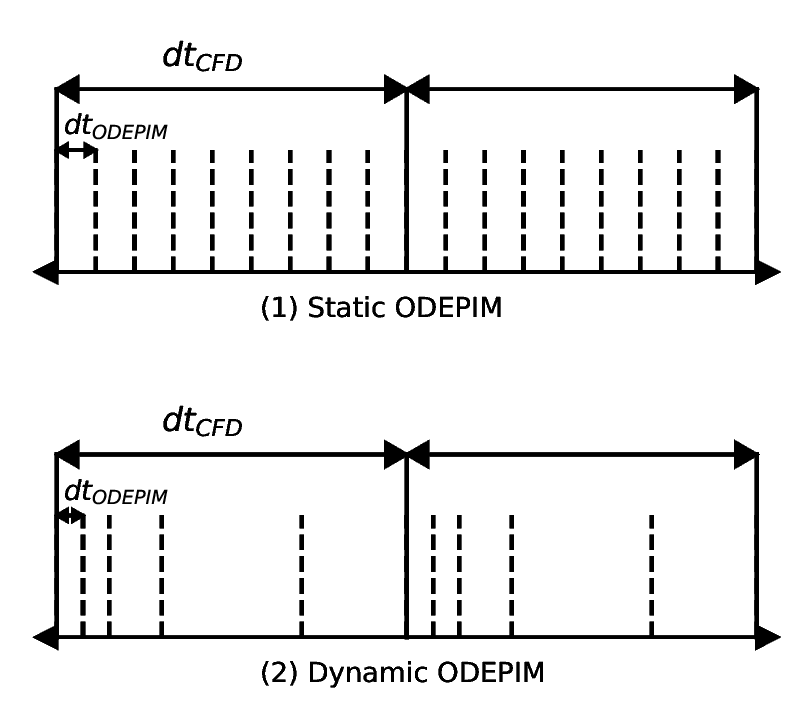
\includegraphics[scale = 0.4]{line.png}
		    \end{minipage}
			
			
		}
		
		%----------------------------------------------------------------------------------------
		%	LOCAL EXTINCTION
		%----------------------------------------------------------------------------------------
		
		\headerbox{Triple Flame \cite{knudsen2012capabilities}}{name=locExt,span=1,column=2,below=flamelet}{ % To reduce this block to 1 column width, remove 'span=2'
			
		    \begin{minipage}{1\linewidth}
		     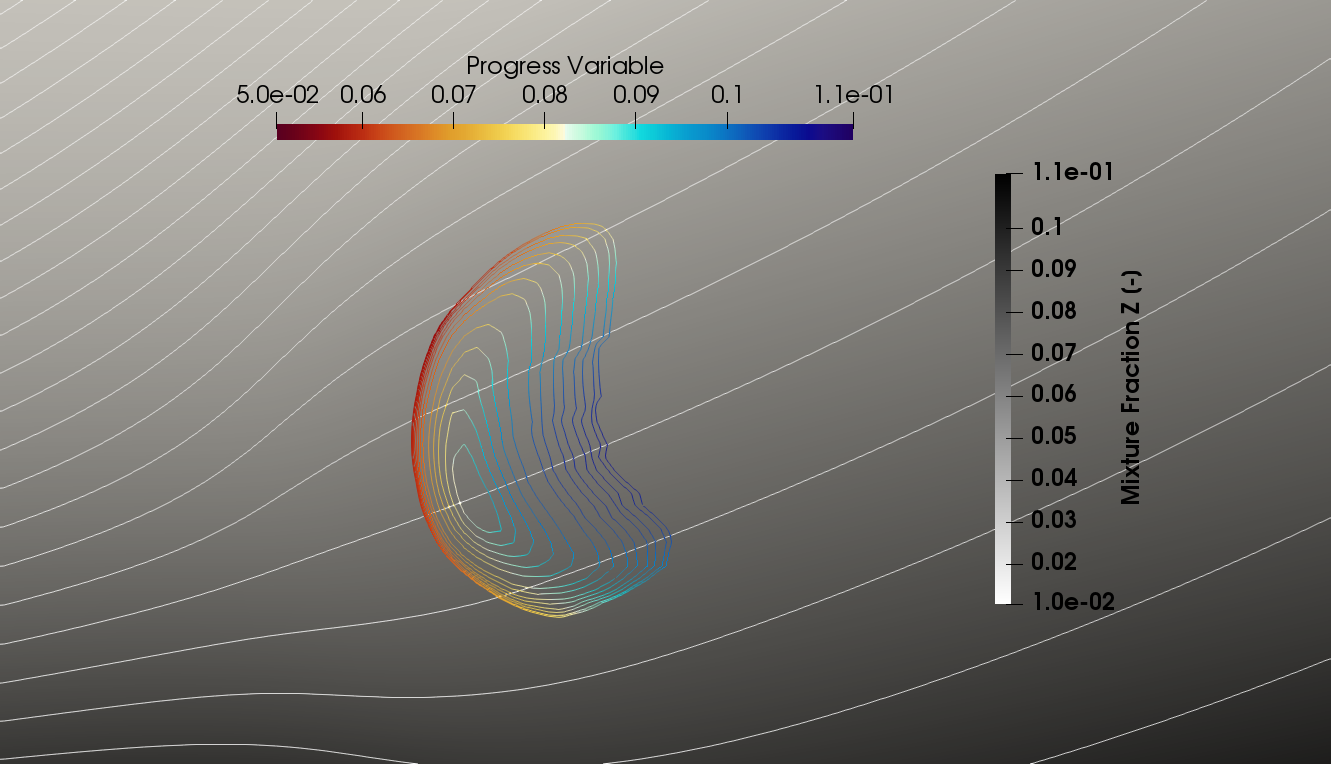
\includegraphics[width=\linewidth]{cont_new.png}
		    \end{minipage}
		    \begin{minipage}{1\linewidth}
		    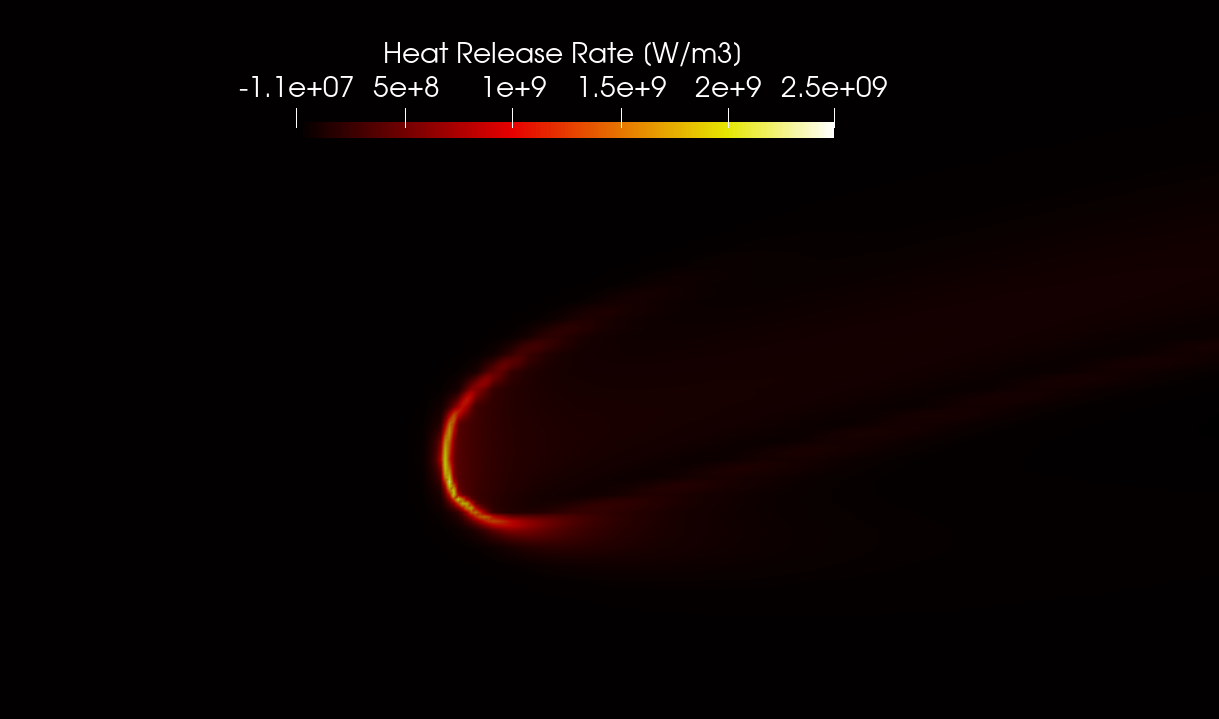
\includegraphics[width=\linewidth]{hrr.png}
		    \end{minipage}
		    \begin{minipage}{1\linewidth}
		      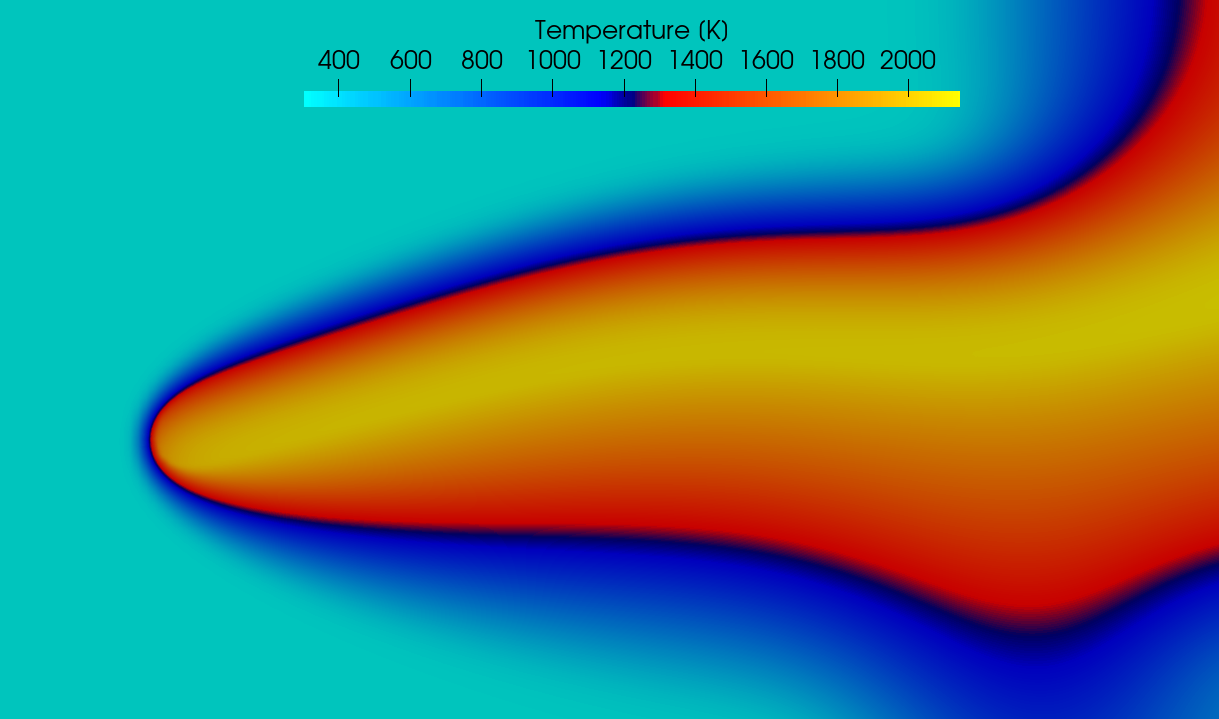
\includegraphics[width=\linewidth]{temp.png}
		    \end{minipage}
		    \begin{minipage}{1\linewidth}
			    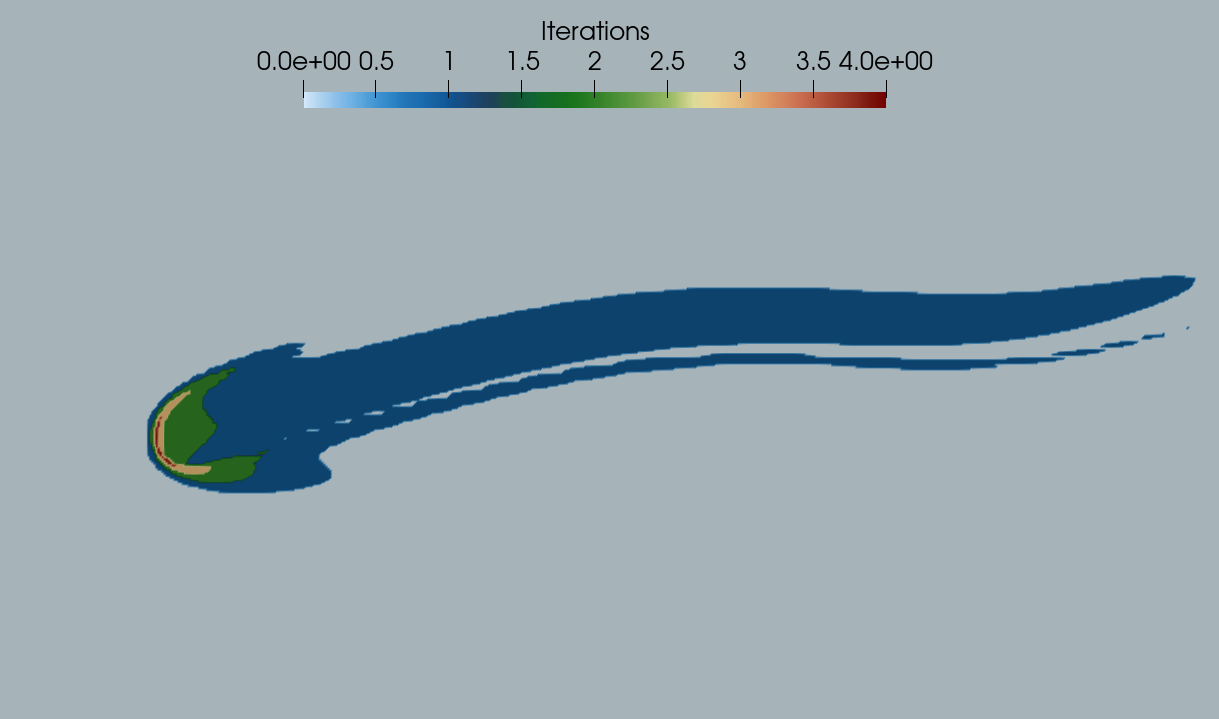
\includegraphics[width=\linewidth]{Odepim.png}
		    \end{minipage}
			
		}	
		
		\headerbox{Triple Flame - Results}{name=tripl,span=1,column=1,below=validation}{ % To reduce this block to 1 column width, remove 'span=2'
			
		
	
		    \begin{minipage}{1.0\linewidth}
		    \centering
			      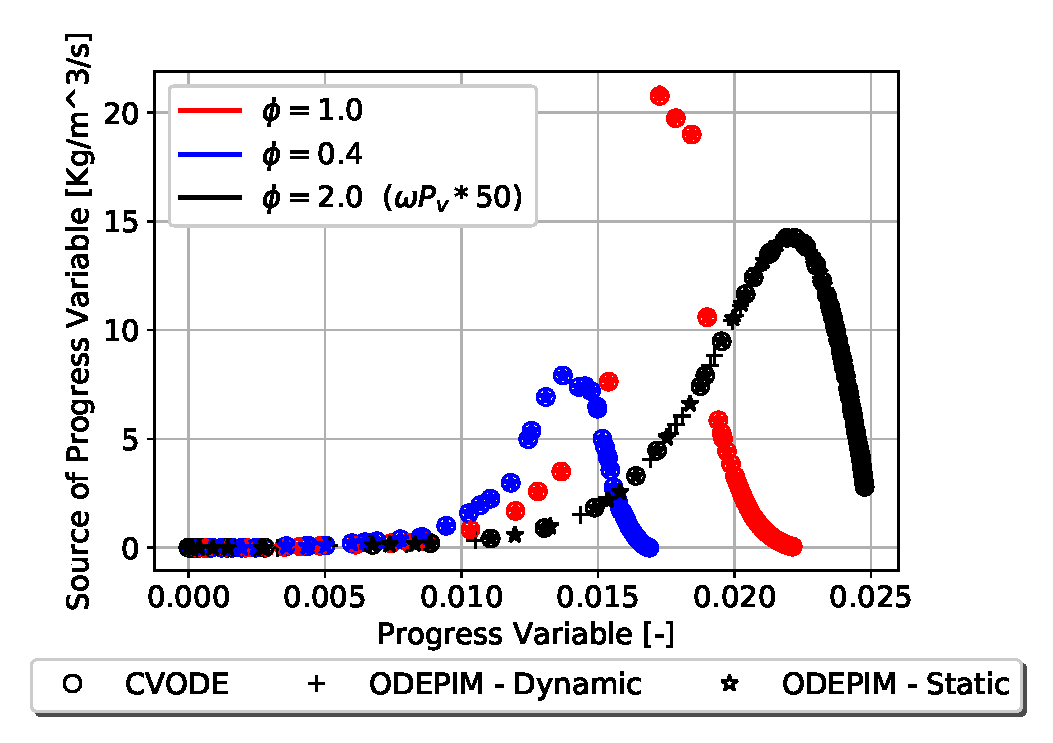
\includegraphics[width=1.0\linewidth]{tri.eps}
			    \\
			     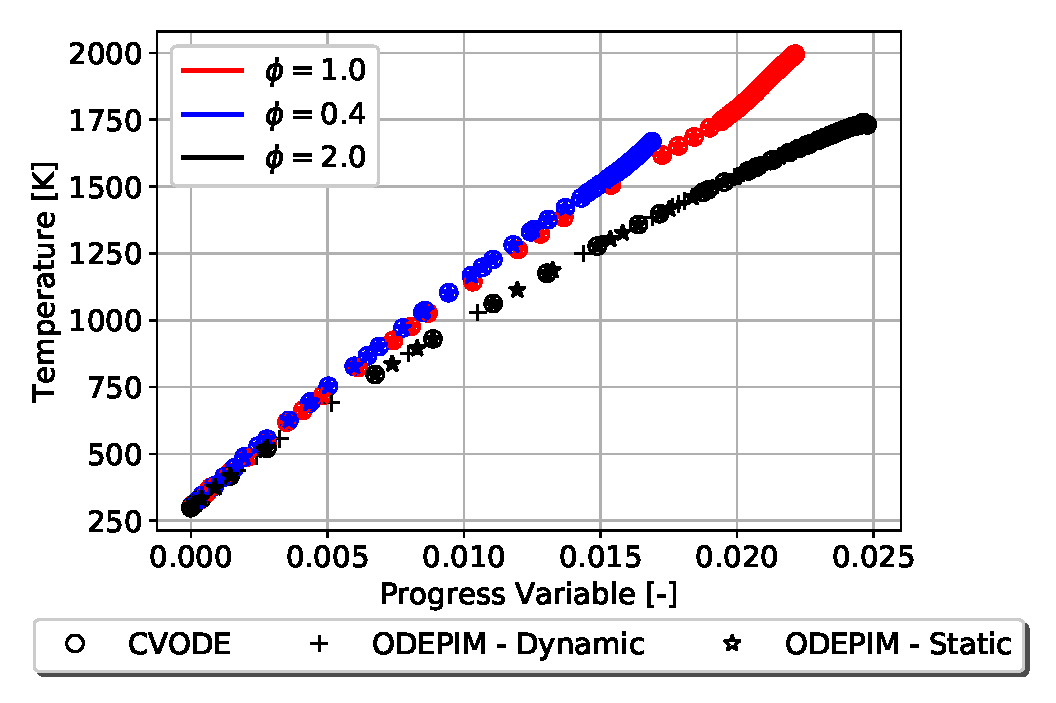
\includegraphics[width=1.0\linewidth]{tri_temp.eps}
		    \end{minipage}
		    }

			
		\headerbox{Acknowledgements}{name=ack,span=1,column=1,below=tripl}{ % To reduce this block to 1 column width, remove 'span=2'
		

		    \begin{minipage}{1.0\linewidth}
			    The research activities conducted here have been financed by the CoEC project from the European Union’s Horizon 2020 research and innovation programme under grant agreement No 952181.
			    \\
			    \\
			    \centering
			    
\includegraphics[width=0.43\linewidth]{COEC_LOGO_RGB-01.png}

		    \end{minipage}
			
			
		}
		
		
		
		
		%----------------------------------------------------------------------------------------
		%	DROPLET MODELLING
		%-----------------------------------------------
		\headerbox{References}{name=references,column=2,below=locExt,span=1}
		{
			\smaller \smaller \smaller % Reduce the font size in this block
			\renewcommand{\section}[2]{\vskip 0.05em} % Get rid of the default "References" section title
			\nocite{*} % Insert publications even if they are not cited in the poster
			
			\bibliographystyle{unsrt}
			\bibliography{sources} % Use sample.bib as the bibliography file
		}
		

	
	\end{poster}
	
\end{document}